\documentclass{beamer}

\usepackage{amsmath, amssymb, amstext}
\usepackage{fancyhdr}
\usepackage{algorithm}
\usepackage{algpseudocode}
\usepackage{mathtools}
\usepackage{tikz}
\usetikzlibrary[topaths]

\DeclarePairedDelimiter{\ceil}{\lceil}{\rceil}
\DeclarePairedDelimiter\floor{\lfloor}{\rfloor}

%Macros
\newcommand{\A}{\mathbb{A}} \newcommand{\C}{\mathbb{C}}
\newcommand{\D}{\mathbb{D}} \newcommand{\F}{\mathbb{F}}
\newcommand{\N}{\mathbb{N}} \newcommand{\R}{\mathbb{R}}
\newcommand{\T}{\mathbb{T}} \newcommand{\Z}{\mathbb{Z}}
\newcommand{\Q}{\mathbb{Q}}
 
 
\newcommand{\cA}{\mathcal{A}} \newcommand{\cB}{\mathcal{B}}
\newcommand{\cC}{\mathcal{C}} \newcommand{\cD}{\mathcal{D}}
\newcommand{\cE}{\mathcal{E}} \newcommand{\cF}{\mathcal{F}}
\newcommand{\cG}{\mathcal{G}} \newcommand{\cH}{\mathcal{H}}
\newcommand{\cI}{\mathcal{I}} \newcommand{\cJ}{\mathcal{J}}
\newcommand{\cK}{\mathcal{K}} \newcommand{\cL}{\mathcal{L}}
\newcommand{\cM}{\mathcal{M}} \newcommand{\cN}{\mathcal{N}}
\newcommand{\cO}{\mathcal{O}} \newcommand{\cP}{\mathcal{P}}
\newcommand{\cQ}{\mathcal{Q}} \newcommand{\cR}{\mathcal{R}}
\newcommand{\cS}{\mathcal{S}} \newcommand{\cT}{\mathcal{T}}
\newcommand{\cU}{\mathcal{U}} \newcommand{\cV}{\mathcal{V}}
\newcommand{\cW}{\mathcal{W}} \newcommand{\cX}{\mathcal{X}}
\newcommand{\cY}{\mathcal{Y}} \newcommand{\cZ}{\mathcal{Z}}

\author{Justin Toth}
\institute{University of Waterloo}
\date{March 1st, 2016}
\title{Stable Matching Polytope\\ and Iterative Rounding}

\begin{document}
\begin{frame}
\titlepage
\end{frame}

\AtBeginSubsection[]
{
	\begin{frame}<beamer>
		\frametitle{Outline}
		\tableofcontents[currentsection, currentsubsection]
	\end{frame}
}
\section{Iterative Rounding}
\subsection{Bipartite Matching}

\begin{frame}
\frametitle{Weighted Bipartite Matching Problem}
Let $G=(V, E)$ be a bipartite graph with bipartition $V = V_0 \dot\cup V_1$. For each edge $e \in E$, assign a cost $c_e$. A matching on $G$ is a subset of edges $M \subseteq E$ such that $\delta(v) \cap M \leq 1$ for all $v \in V$. We will say $M(v)$ denotes the vertex $v \in V$ is matched to under $M$. The weighted bipartite matching problem is to find a matching $M$ maximizing $\sum_{e\in M} c_e$.

\begin{figure}
\centering
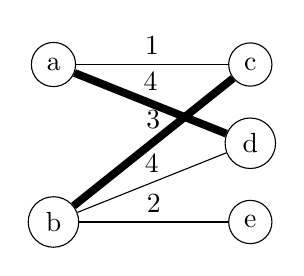
\begin{tikzpicture}
   \node[shape=circle,draw=black] (B) at (0,1) {b};
    \node[shape=circle,draw=black] (A) at (0,3) {a};
    \node[shape=circle,draw=black] (E) at (2.5,1) {e};
    \node[shape=circle,draw=black] (D) at (2.5,2) {d}; 
    \node[shape=circle,draw=black] (C) at (2.5,3) {c};

    \path[-] (A) edge node[above] {$1$} (C);
    \path [line width=1mm,-](A) edge node[above] {$4$} (D);
    \path [line width=1mm,-](B) edge node[above] {$3$} (C);
    \path [-](B) edge node[above] {$2$} (E);
    \path [-](B) edge node[above] {$4$} (D);

\end{tikzpicture}
\caption{A bipartite graph with edge weights. Optimal matching edges are thicker. $M(a) = d$}
\end{figure}
\end{frame}

\begin{frame}
\frametitle{Linear Programming Relaxation}
This problem can be formulated as a linear program, denoted $LP_M(G)$:
\begin{align*}
&\text{maximize} &\sum_{e \in E} c_e x_e \\
&\text{subject to} &x(\delta(v)) &\leq 1, &\forall v \in V\\
& &x_e &\geq 0, &\forall e \in E
\end{align*}
Where $x(\delta(v)) = \sum_{e \in \delta(v)} x_e$.
\end{frame}

\subsection{Iterative Rounding Proof Strategy}
\begin{frame}
\frametitle{Why use Iterative Rounding?}
\begin{itemize}
\item Widely applicable to many standard problems such as matchings, spanning trees, network flows
\item Disciplined and (relatively) simple arguments
\item Highly extensible, including to NP-hard variants to achieve approximation algorithms
\end{itemize}
\end{frame}

\begin{frame}
\frametitle{Iterative Rounding Strategy}
Three steps:
\begin{enumerate}
\item<1-> $\textbf{Characterize Extreme Point Solution:}$ Bound any maximal set of linearly independent tight constraints using the Rank Lemma.
\item<2-> $\textbf{Iterative Algorithm:}$ Create an algorithm which constructs an integral solution from an optimal extreme point by fixing variables valued $1$, dropping variables valued $0$, and solving the residual problem on the fractional variables.
\item<3-> $\textbf{Analyze:}$ Show that algorithm correctly solves the problem and the solution returned has value at least (in the case of maximization) as good as the optimal solution to the Linear Programming Relaxation. 
\end{enumerate}
\uncover<1->{$\textbf{Rank Lemma:}$ The maximal number of linearly independent tight constraints at an extreme point is equal to the number of variables.}
\end{frame}

\begin{frame}
\frametitle{What do we get from this?}
With such an algorithm in hand, integrality of the polytope in question is immediate:
\begin{itemize}
\item  It is known from Linear Programming theory that for any extreme point there is a cost vector $c$ for which that extreme point is the unique optimal solution
\item If we had a fractional extreme point, and ran the algorithm with the cost vector for which it is supposedly unique we would obtain an integral solution of equivalent cost
\item Since the integral solution is feasible and clearly not equal to a fractional solution this contradictions uniqueness
\end{itemize}
\end{frame}

\subsection{Proof of Integrality for Bipartite Matching Polytope}
\begin{frame}
\frametitle{Characterize Extreme Point Solution}
Recall that $LP_M(G):$
\begin{align*}
&\text{maximize} &\sum_{e \in E} c_e x_e \\
&\text{subject to} &x(\delta(v)) &\leq 1, &\forall v \in V\\
& &x_e &\geq 0, &\forall e \in E
\end{align*}
Let $x$ be an extreme point of $LP_M(G)$ such that $0<x<1$. Then there exists a set $W \subseteq V$ such that:
\begin{enumerate}
\item $|W| = |E|$
\item $x(\delta(v)) = 1$ for all $v \in W$
\item $\{\chi(\delta(v)) : v \in W \}$ is linearly independent
\end{enumerate}
where $\chi(\delta(v))$ denotes the incidence vector of $\delta(v)$.
\end{frame}

\begin{frame}
\frametitle{Iterative Algorithm}
\begin{enumerate}
\item Input bipartite matching instance $G$
\item Set matching $M$ to $\emptyset$
\item While $E \neq \emptyset$
\begin{enumerate}
\item Find extreme point optimal solution $x$ to $LP_M(G)$.
\item For each $e=vw \in E$ such that $x_e = 1$ add $e$ to $M$ and remove vertices $v,w$ from $G$.
\item For each $e \in E$ such that $x_e = 0$ remove $e$ from $G$.
\end{enumerate}
\item Output $M$
\end{enumerate}
\end{frame}

\begin{frame}
\frametitle{Correctness - Finding $0$ or $1$}
\begin{itemize}
\item<1-> Suppose for contradiction we have an extreme point solution $x$ such that $0 < x < 1$
\item<2-> By our characterization we may find $W \subseteq V$ of size $|E|$ corresponding to a set of tight linearly independent constraints.
\item<3-> Give a token to each edge $vw$. Then have it give $\frac{1}{2}$ token to $v$ if $v \in W$ and have it give $\frac{1}{2}$ token to $w$ if $w \in W$. 
\item<4->Remains to show that after redistribution each constraint in $W$ has at least $1$ token and some edge has a remaining fractional token.
\end{itemize}
\end{frame}
\begin{frame}
\frametitle{Correctness - Finding $0$ or $1$ continued}
\begin{itemize}
\item<1-> Clearly each edge does not give away more tokens than it has
\item<2-> For any $v \in W$, $x(\delta(v)) = 1$, and since $x_e < 1$ for each $e \in \delta(v)$ we have that the degree of $v$, $d(v)$, is at least $2$.
\item<3-> Thus each tight constraint receives at least $1$ token.
\item<4-> Since $\sum_{v \in V_0} \chi(\delta(v)) = \sum_{v \in V_1} \chi(\delta(v))$ by bipartiteness, there is a vertex $v \not\in W$ (otherwise constraints in $W$ are not linearly independent).
\item<5-> Any edge incident on said $v$ does not give away all its tokens. So $|E| > |W|$, a contradiction.
\end{itemize}
\end{frame}

\begin{frame}
\frametitle{Correctness - Optimality}
\begin{itemize}
\item<1-> We will show the algorithm returns a matching of cost at least that of the optimal solution to $LP_M(G)$ by induction on the number of iterations of the algorithm.
\item<2-> If the algorithm fixes $x_{vw} = 1$ during an iteration then the residual problem is to find a matching $M'$ on $G'=G-v-w$. Then $M' \cup \{vw\}$ is the matching returned by the algorithm.
\item<3-> The vector $x' = x$ restricted to the edges of $G'$ is feasible for $LP_M(G')$.
\item<4-> Therefore $c(M' \cup \{vw\}) = c(M') + c_{vw} \geq c(x') + c_{vw} = c(x)$,
\item<5-> The case for fixing $x_{vw} = 0$ is similar.
\end{itemize}
\end{frame}

\section{Stable Matching Polytope}
\subsection{Problem Formulation}
\begin{frame}
\frametitle{Stable Matching Problem}
\begin{itemize} \item As before consider a weighted bipartite graph $G$. But now each vertex ranks their neighbours in order of preference. \item So for any two neighbours $w_1, w_2$ of $v$ we write $w_1 >_v w_2$ to denote that $v$ prefers $w_1$ to $w_2$. \item For any neighbour $w$ of $v$ we let $\delta^{>w}(v) = \{vw' \in E : w' >_v w\}$. \item Let $n^*(v)$ ($n_*(v)$ respectively) denote the most (least respectively) preferred neighbour of $v$. \end{itemize} We aim to find a max weight stable matching.
\end{frame}

\begin{frame}
\frametitle{Stability}
A matching $M$ on $G$ is said to be stable if there does not exist $vw \in E$ (called a blocking pair) for which any of the following holds:
\begin{enumerate}
\item Both $v$ and $w$ have matches and $M(v) <_v w$ and $M(w) <_w v$ \\
\item $v$ has a match but not $w$ and $M(v) <_v w$\\
\item $w$ has a match but not $v$ and $M(w) <_w v$\\
\item Both $v$ and $w$ have no matches
\end{enumerate}
\end{frame}

\begin{frame}
\frametitle{A blocking pair}
Suppose that in the graph below, $c >_a d$ and $a >_c b$. Then $ac$ is a blocking pair.
\begin{figure}
\centering
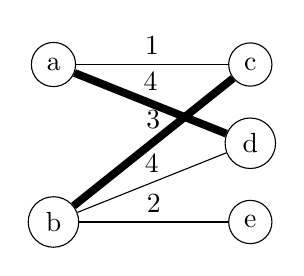
\begin{tikzpicture}
   \node[shape=circle,draw=black] (B) at (0,1) {b};
    \node[shape=circle,draw=black] (A) at (0,3) {a};
    \node[shape=circle,draw=black] (E) at (2.5,1) {e};
    \node[shape=circle,draw=black] (D) at (2.5,2) {d}; 
    \node[shape=circle,draw=black] (C) at (2.5,3) {c};

    \path[-] (A) edge node[above] {$1$} (C);
    \path [line width=1mm,-](A) edge node[above] {$4$} (D);
    \path [line width=1mm,-](B) edge node[above] {$3$} (C);
    \path [-](B) edge node[above] {$2$} (E);
    \path [-](B) edge node[above] {$4$} (D);

\end{tikzpicture}
\caption{This matching has a blocking pair $ac$.}
\end{figure}
\end{frame}

\begin{frame}
\frametitle{A Linear Programming Relaxation}
Let $LP_{SM}(G)$ be defined as follows:
\begin{align*}
&\text{maximize} &\sum_{e \in E} c_e x_e \\
&\text{subject to} &x(\delta(v)) &\leq 1, &\forall v \in V\\
& &x(\delta^{>w}(v)) + x(\delta^{>v}(w)) + x_{vw} &\geq 1, &\forall vw \in E\\
& &x_e &\geq 0, &\forall e \in E
\end{align*}
For any $v \in V$, similar to $n^*(v)$ we will let $n^*(x,v)$ ($n_*(x,v)$ respectively) denote the most (least respectively) preferred neighbour of $v$ such that $x_{vn^*(x,v)} > 0$ ($x_{vn_*(x,v)} > 0$ respectively). \\
Also define $S(x) = \{ v \in V : x(\delta(v)) > 0 \}$.
\end{frame}

\subsection{Some Observations}
\begin{frame}
\frametitle{Integral Points are Stable}
Let $x$ be the incidence vector of a matching on $G$. Then $x$ is stable if and only if $x$ is feasible for $LP_{SM}(G)$.\\
$\textbf{Proof Idea:}$ Since $x$ is integral, $x$ is infeasible if and only if there exists $vw \in E$ such that $$ x(\delta^{>w}(v)) = x(\delta^{>v}(w)) = x_{vw} = 0. $$
Such a $vw$ is a blocking pair. $\blacksquare$
\end{frame}

\begin{frame}
\frametitle{Lemma 1}
Let $x$ be feasible for $LP_{SM}(G)$ and let $vw \in E$. Then $$ v \not\in S(x) \text{ or } (vw \in S(x) \text{ and } w \geq_v n^*(x,v)) $$ implies that $$ x(\delta(w)) = 1 \text{ and } v \leq_w n_*(x,w). $$\\
$\textbf{Proof Idea:}$ In either case $x(\delta^{>w}(v)) = 0$. So $$1 \leq x(\delta^{>w}(x)) + x(\delta^{>v}(w)) + x_{vw} = x(\delta^{\geq v}(w)) \leq 1. \blacksquare$$\\
$\textbf{Note:}$ If $x(\delta^{>w}(v)) + x(\delta^{>v}(w)) + x_{vw} = 1$ then the converse of Lemma $1$ holds as well.
\end{frame}

\begin{frame}
\frametitle{Lemma 2}
Let $x$ be feasible for $LP_{SM}(G)$ and let $vw \in E$. Then $$v \in S(x) \text{ and } w = n^*(x,v)$$ if and only if $$x(\delta(w)) = 1 \text{ and } v = n_*(x,w). $$\\
$\textbf{Proof Idea:}$ Similar to previous with equality holding throughout. $\blacksquare$
\end{frame}

\begin{frame}
\frametitle{Lemma 3}
Let $x$ be feasible for $LP_{SM}(G)$. Then $$ v \in S(x) $$ if and only if $$x(\delta(v)) = 1.$$ \\
$\textbf{Proof Idea:}$ We establish a bijection between $S(x)$ and $F(x) = \{v \in V : x(\delta(v)) = 1\}$. Clearly $F(x) \subseteq S(x)$ so it is enough to show a one-to-one (injective) map. In fact, $n^*(x,\cdot)$ is such a map. If $n^*(x,v_1) = w = n^*(x,v_2)$ then by Lemma $2$ $v_1 = n_*(x,w) = v_2$. $\blacksquare$
\end{frame}

\subsection{Rothblum's Original Proof}
\begin{frame}
\frametitle{Proof of Integrality}
Rothblum showed that the extreme points of  $LP_{SM}(G)$:
\begin{align*}
&\text{maximize} &\sum_{e \in E} c_e x_e \\
&\text{subject to} &x(\delta(v)) &\leq 1, &\forall v \in V\\
& &x(\delta^{>w}(v)) + x(\delta^{>v}(w)) + x_{vw} &\geq 1, &\forall vw \in E\\
& &x_e &\geq 0, &\forall e \in E
\end{align*}
are integral.\\
One direction is easy. If we have an integral feasible solution of $LP_{SM}(G)$ then it is extreme since the solutions of $LP_{SM}(G)$ are contained in the solutions of $LP_M(G)$ which we have already shown has integral extreme point solutions.
\end{frame}

\begin{frame}
\frametitle{Proof of Integrality - Strategy}
Now suppose that we have an extreme point solution $x$ to $LP_{SM}(G)$. Rothblum uses a convex combination argument to achieve integrality. 
\begin{itemize}
\item Recall that $x$ is an extreme point if and only if there does not exist $x^1 \neq x^2$ feasible solutions such that $x = \frac{1}{2}(x^1 + x^2)$.
\item Rothblum elegantly defines a vector $z$ such that $z = 0$ implies that for all $v \in V$, $n^*(x,v) = n_*(x,v)$ and thus $x$ is integral (each $x(\delta(v)) = 1$ or $0$ and there is at most one non-zero edge incident to each $v$).
\item Rothblum then shows $x = \frac{1}{2}(x + \epsilon z  + x - \epsilon z)$ for sufficiently small $\epsilon$ and by extremality of $x$ the proof is complete.
\end{itemize}
\end{frame}

\begin{frame}
\frametitle{Proof of Integrality - Definition of $z$}
Define the vectors $z^*$, $z_*$, and $z$ as follows:
\begin{align*}
(z^*)_{vw} &= \begin{cases}
	1, &\text{if $v\in S(x) \cap V_0$ and $w = n^*(x,v)$} \\
	0, &\text{otherwise}
\end{cases} 
\\
\uncover<2->{(z_*)_{vw} &= \begin{cases}
	1, &\text{if $v\in S(x) \cap V_0$ and $w = n_*(x,v)$} \\
	0, &\text{otherwise}
\end{cases}}
\\
\uncover<3->{z_{vw} &= (z^*)_{vw} - (z_*)_{vw}.}
\end{align*}
\uncover<4->{By invoking our Lemmas, $z^*$ and $z_*$ are equivalently:
\begin{align*}
(z^*)_{vw} &= \begin{cases}
	1, &\text{if $w\in S(x) \cap V_1$ and $v = n_*(x,w)$} \\
	0, &\text{otherwise}
\end{cases} 
\\
(z_*)_{vw} &= \begin{cases}
	1, &\text{if $w\in S(x) \cap V_1$ and $v = n^*(x,w)$} \\
	0, &\text{otherwise}
\end{cases}
\end{align*}}
\end{frame}

\begin{frame}
\frametitle{Proof of Integrality - Showing $x \pm \epsilon z$ is Feasible}
We claim that $z$ satisfies the following:
\begin{itemize}
\item<2-> If $x(\delta(v)) = 1$ then $z(\delta(v)) = 0$ for all $v \in V$.
\item<3-> If $x_e = 0$ then $z_e = 0$ for all $e \in E$.
\item<4-> If $x(\delta^{>w}(v)) + x(\delta^{>v}(w)) + x_{vw} = 1$ then $z(\delta^{>w}(v)) + z(\delta^{>v}(w)) + z_{vw} = 0$.
\end{itemize}
\uncover<5->{That is to say $z$ is in the null space of the matrix of constraints tight at $x$. Thus we can choose $\epsilon > 0$ such that $x \pm \epsilon z$ is feasible for $LP_{SM}(G)$}. \\
\uncover<6->{Since $x$ is an extreme point this means $z = 0$. That is, $z^* = z_*$. So each $v \in V$ that is matched has one non-zero incident edge. Further by our Lemmas each such $v$ satisfies $x(\delta(v)) = 1$ and therefore $x$ is integral. $\blacksquare$}
\end{frame}

\section{An Iterative Rounding Proof?}
\subsection{Extreme Point Characterization}
\begin{frame}
Recall: $LP_{SM}(G)$:
\begin{align*}
&\text{maximize} &\sum_{e \in E} c_e x_e \\
&\text{subject to} &x(\delta(v)) &\leq 1, &\forall v \in V\\
& &x(\delta^{>w}(v)) + x(\delta^{>v}(w)) + x_{vw} &\geq 1, &\forall vw \in E\\
& &x_e &\geq 0, &\forall e \in E
\end{align*}
We ask if there exists an Iterative Rounding based proof of integrality?\\
Recall Iterative Rounding: \\Characterize tight constraints $\Rightarrow$ Iterative Algorithm $\Rightarrow$ Analysis.
\end{frame}

\begin{frame}
\frametitle{Extreme Point Characterization}
Let $x$ be an extreme point solution to $LP_{SM}(G)$ such that $x>0$. Then there exists $W \subseteq V$ and $T \subseteq E$ such that the following hold:
\begin{enumerate}
\item $x(\delta(v)) = 1$, $\forall v \in W$.
\item $x(\delta^{>w}(v))+ x(\delta^{>v}(w) + x_{vw} = 1$, $\forall vw \in T$.
\item The vectors in $\{\chi(\delta(v)) : v \in W\}$ together with the vectors in $\{\chi(\delta_v^>(w)) + \chi(\delta_w^>(v)) + \chi(vw) : vw \in T\}$ are all linearly independent.
\item $|W| + |T| = |E|$.
\end{enumerate}
$\textbf{Proof:}$ Immediate from Rank Lemma (The maximal number of linearly independent tight constraints at an extreme point is equal to the number of variables). $\blacksquare$
\end{frame}
\subsection{Finding a $0$ or $1$}
\begin{frame}
\frametitle{Finding a $0$ or $1$ - Choose $W$ and $T$}
Suppose for a contradiction we have an extreme point solution of $LP_{SM}(G)$, $x$, such that $0 < x < 1$. We may choose $W \subseteq V$ and $T \subseteq E$ corresponding to a maximal set of linearly independent tight constraints such that $|W| + |T| = |E|$. Choose the pair $(W,T)$ which  maximizes $|W|$.\\
\uncover<2->{
As before, for any $v \in W$, $d(v) \geq 2$.\\
$\textbf{Proof Idea:}$ $x(\delta(v)) = 1$ and $x_e < 1$ for each $e \in \delta(v)$ so $d(v) \geq 2$. }
\end{frame}
\begin{frame}
\frametitle{Finding a $0$ or $1$ - degree of $v \in W$}
The following claims show that each tight vertex $v \in W$ has two adjacent edges not in $T$:
\begin{itemize}
\item<2-> Let $v \in W$.  Let $w = n_*(v)$. Then $vw \not\in T$. \\
$\textbf{Proof Idea:}$ If $vw$ in $T$ then since $\delta^{\geq w}(v) = \delta(v)$ we have that $\chi(\delta^{>w}(v)) + \chi(\delta^{>v}(w)) + \chi(vw) = \chi(\delta(v))$ this contradicts the linear independence of the constraints chosen.
\item<3-> Let $v \in V$. Let $w = n^*(v)$. Then $vw \not\in T$. \\
$\textbf{Proof Idea:}$ If $vw \in T$ then $x(\delta^{\geq v}(w)) = 1$. So $\chi(\delta^{\geq v}(w)) = \chi(\delta(w))$ and $\chi(\delta^{>w}(v)) + \chi(\delta^{>v}(w)) + \chi(vw) = \chi(\delta(w)).$ If $w \in W$ this contradicts linear independence. Otherwise this contradicts the maximality of $W$.
\end{itemize}
\end{frame}
\begin{frame}
\frametitle{Finding a $0$ or $1$ - Token argument}
Give each edge in $E$ a token and have them distribute tokens to the tight constraints as follows for any $vw \in E$:
\begin{enumerate}
\item If $vw \in T$ have $vw$ give itself token.
\item Otherwise if $v \in W$ have $vw$ give $\frac{1}{2}$ token to $v$, and if $w \in W$ have $vw$ give $\frac{1}{2}$ token to $w$.
\end{enumerate}
\begin{itemize}
\item<2-> Clearly each edge does not give away more than it has, and each edge in $T$ receives a token.
\item<3-> Each vertex in $W$ receives a token since there are at least two adjacent edges not in $T$. 
\item<4-> As in the bipartite matching argument, we can find $v \not\in W$ and the edge $vn^*(v)$ does not give away all of its token. 
\end{itemize}
\uncover<4->{A contradiction.$\blacksquare$}
\end{frame}
\subsection{Algorithm?}
\begin{frame}
\frametitle{Iterative Algorithm}
\begin{enumerate}
\item Input bipartite stable matching instance $G$
\item Set matching $M$ to $\emptyset$
\item While $E \neq \emptyset$
\begin{enumerate}
\item Find extreme point optimal solution $x$ to $LP_M(G)$.
\item For each $e=vw \in E$ such that $x_e = 1$ add $e$ to $M$ and remove vertices $v,w$ from $G$.
\item For each $e \in E$ such that $x_e = 0$ remove $e$ from $G$.
\end{enumerate}
\item Output $M$
\end{enumerate}
\uncover<2->{But this doesn't work!\\ $LP_{SM}(G-e)$ loses the stability constraint for $e$ so the stable matching returned by the algorithm on $G-e$, $M'$, is not necessarily such that $M' \cup \{e\}$ is a stable matching on $G$}
\end{frame}
\begin{frame}
\frametitle{Can We Fix The Algorithm? - Edges of value $1$}
When we find $x_{vw} = 1$ we can be clever and do the following:
\begin{enumerate}
\item $\forall u \in N(v)$ (the neighbourhood of $v$) such that $v$ prefers $u$ to $w$ remove every edge in $\delta_u^<(v)$ from $G$
\item $\forall u \in N(w)$ such that $w$ prefers $u$ to $v$ remove every edge in $\delta_u^<(w)$ from $G$.
\item Remove $v, w$ from $G$.
\end{enumerate}
It can be shown that this ensures the matching returned on the residual graph plus edge $vw$ is a stable matching on $G$.\end{frame}
\begin{frame}
\frametitle{Can We Fix The Algorithm? - Edges of value $0$}
Unfortunately it is not clear what to do in the case where edges of value $0$ are found.\\
Questions to think about:
\begin{itemize}
\item Can we guarantee an edge of value $1$ to avoid this?
\item Is there a clever set of edges to remove alongside a $0$ edge to ensure the algorithm works?
\end{itemize}
\end{frame}
\section{References}
\begin{frame}
\frametitle{References}
\begin{enumerate}
\item Rothblum, Uriel G. "Characterization of stable matchings as extreme points of a polytope." $\textit{Mathematical Programming}$ 54.1-3 (1992): 57-67.
\item Lau, Lap Chi, Ramamoorthi Ravi, and Mohit Singh. $\textit{Iterative methods in combinatorial optimization}$. Vol. 46. Cambridge University Press, 2011
\end{enumerate}
\end{frame}
\end{document}
